\section{Discussion}

In this work, we sought to objectively compare the robustness and user
preference of the neuromuscular and impedance control strategies for powered,
robotic knee and ankle prostheses. Overall, we found that users rated the
neuromuscular control more highly than impedance control and using impedance
control led to significantly more falls compared to walking without a
prosthesis. While the median number of falls accrued by impedance control across
all subjects in both the undisturbed and disturbed conditions was higher than
those of neuromuscular control, these differences were not significant. The only
measure of gait stability in which a significant difference between the
neuromuscular and impedance controllers was measured was the torso pitch
variability, which neuromuscular control significantly reduced in the
disturbance case compared to impedance control.

Categorizing the falls by their type gives more insight into differences between
the controllers. There were reasons for falls with each controller that did not
exist for the other. For NM control, missed transitions between stance and swing
caused three falls. While these falls could be directly attributed to the
leg-angle threshold in the high level state machine that governs the
stance/swing state transition (\cref{fig:stance_swing_state_machine}), that
these falls only occurred with neuromuscular control suggests a causal
difference in the two strategies. One possible important difference between the
implemented neuromuscular and impedance control strategies was that impedance
control typically provided much more ankle push of work, as shown in
\cref{fig:treadmill_exp_ankle_work}. In impedance control, the transition
transition to the third phase of gait generates a large burst of ankle power,
which users may interpret as a signal that the prosthesis is ready to enter
swing. In contrast, neuromuscular control may not have provided any such signal
due to the lack of ankle work. It is possible that such cues to the user should
be explicitly considered in the design of prosthesis controllers, especially
when they can help inform correct transition of discrete state.
\begin{marginfigure}
    \centering 
    %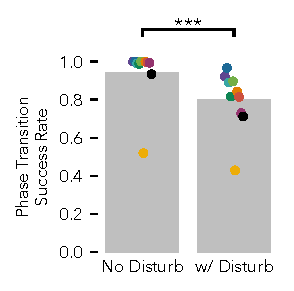
\includegraphics[width=\textwidth]{phase_success}
    \missingfigure[figwidth=\textwidth]{ankle work}
    \caption{Normal Walking, impedance and neuromuscular control ankle
    work.}\label{fig:treadmill_exp_ankle_work}
\end{marginfigure}

Impedance control suffered from two failure modes specific to the structure of
its stance finite state machine. The first failure mode, missed transitions
between the second and third phases of stance occurred if the user did not
dorsiflex the ankle enough to trigger the transition. This failure could often
lead to trips during swing or a later loss of balance. In contrast, the knee
collapse failure mode happened if the impedance controller switched to the third
phase of stance too early, which could cause a sudden reduction in knee
extension torque. The fact that individual subjects fell for both of these
reasons suggests that these failure modes cannot simply fixed by tuning the
ankle angle threshold. Decreasing the threshold to prevent missed transitions
would likely cause more knee collapses. Conversely, increasing the threshold
would likely cause more missed transitions. This problem of correctly estimating
phase during stance motivates the work we present in \cref{sec:phase_estimation}
in which we derive a control based on a more robust estimate of stance.

Users suffered from trips during swing when using both stance control
strategies, which were both paired with the same minimum-jerk trajectory
generation swing control strategy. However, these trips occurred three times
more frequently with impedance stance control than with neuromuscular stance
control. Many of the trips that occurred with impedance control were preceded by
a missed transition between the second and third stance phases. Neuromuscular,
control, in contrast, is smooth throughout stance with no discrete transitions,
and thus may allow for a smoother transition to swing and fewer swing trips. In
\cref{sec:swing_control_planning} we seek to explicitly minimize the risk of
falling by using an estimate of the current and future trajectories of the hip
height and orientation to plan knee and ankle swing trajectories that avoid
premature ground contact.

Control complexity 

Whats going on with suboptimal params


